\chapter{Trustworthy AI in the EU}


\begin{remark}
    The European Commission's vision for artificial intelligence is based on three pillars:
    \begin{enumerate}
        \item Increase public and private investments,
        \item Prepare for socio-economic changes (e.g., protect who gets substituted with AI),
        \item Ensure a proper ethical and legal framework to strengthen European values.
    \end{enumerate}
\end{remark}



\section{AI4People's Ethical Framework for a Good AI Society}

\begin{description}
    \item[AI for people (AI4People)] \marginnote{AI for people (AI4People)}
        Multi-stakeholder forum created in 2018 with the goal of defining the founding principles, policies, and practices to build a ``good AI society''.

    \item[Ethical Framework for a Good AI Society] \marginnote{Ethical Framework for a Good AI Society}
        White paper that:
        \begin{enumerate}
            \item Identifies opportunities of AI on society and its risks.
            \item Defines the guiding principles for AI.
            \item Presents recommendations for a good AI society.
        \end{enumerate}
\end{description}


\subsection{Opportunities and risks of AI for society}

This chapter identifies four opportunity-risk points of AI systems:
\begin{descriptionlist}
    \item[Enable self-realization] \marginnote{Enable self-realization} (``who we can become'')
        AI systems can automate mundane aspects of life and leave more free time for cultural, intellectual, and social activities. However, this should not devalue human skills.

    \item[Enhance human agency] \marginnote{Enhance human agency} (``what we can do'')
        AI systems can enhance human decision-making. However, it should not lift humans from responsibilities.

    \item[Increase societal capabilities] \marginnote{Increase societal capabilities} (``what we achieve'')
        AI systems can support in solving problems and achieving goals. However, they should still be supervised by humans.

    \item[Cultivate societal cohesion] \marginnote{Cultivate societal cohesion} (``how can we interact with each other and the world'')
        AI systems can support in coordinating complex problems that require societal cohesion. However, its decisions should not undermine human self-determination.
\end{descriptionlist}

\begin{figure}[H]
    \centering
    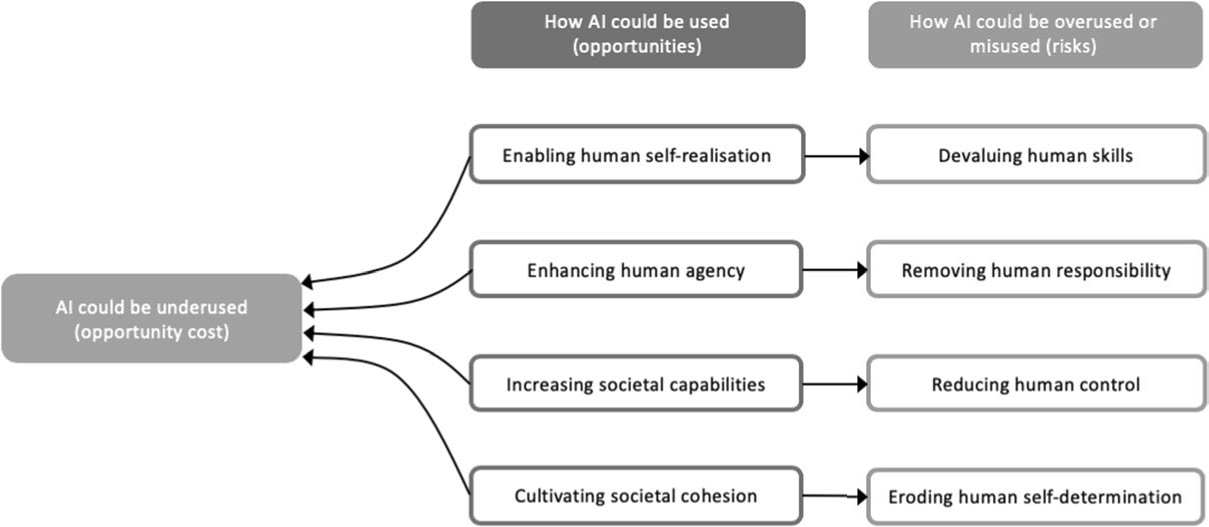
\includegraphics[width=0.65\linewidth]{./img/ai4people_opportunities_risks.png}
\end{figure}


\subsection{Unified framework of principles for AI in society}

This chapter groups and presents the common principles used by different organizations and initiatives.

Most of them overlap with the principles of bioethics:
\begin{descriptionlist}
    \item[Beneficence] \marginnote{Beneficence}
        AI should be created to benefit humanity.

    \item[Non-maleficence] \marginnote{Non-maleficence}
        AI systems should not cause harm.
    
    \item[Autonomy] \marginnote{Autonomy}
        There should be a balance between the decision-making power we delegate to an AI system and the one we keep.
    
    \item[Justice] \marginnote{Justice}
        AI systems should contribute to global justice and equality.
\end{descriptionlist}

In addition, an AI specific principle is added:
\begin{descriptionlist}
    \item[Explicability] \marginnote{Explicability}
        AI systems should be understandable and their decisions accountable.
\end{descriptionlist}


\subsection{Recommendations for a good AI society}

This chapter presents 20 action points of four types:
\begin{description}
    \item[Assessment] \phantom{}
        \begin{itemize}
            \item Assess the capabilities of existing institutions in dealing with harms caused by AI systems.
            \item Assess which task should not be delegated to AI systems.
            \item Assess whether current regulations are sufficiently grounded in ethics.
        \end{itemize}

    \item[Development] \phantom{}
        \begin{itemize}
            \item Develop a framework to enhance AI systems' explicability.
            \item Develop adequate legal procedures to evaluate AI decisions.
            \item Develop auditing mechanisms for AI systems to deal with unfairness and risks.
            \item Develop a mechanism to fix or compensate AI mistakes.
            \item Develop metrics for trustworthiness of AI systems.
            \item Develop an EU oversight agency to evaluate AI systems.
            \item Develop a European observatory for AI.
            \item Develop legal instruments and contractual templates.
        \end{itemize}
        
    \item[Incentivization] \phantom{}
        \begin{itemize}
            \item Incentivize the development of AI systems that are socially preferable and environmentally friendly.
            \item Incentivize European research.
            \item Incentivize cross-disciplinary and cross-sectoral cooperation.
            \item Incentivize the inclusion of ethical, legal, and social considerations in AI research.
            \item Incentivize the development of de-regulated testing zones for AI systems.
            \item Incentivize research about public perception and understanding of AI.
        \end{itemize}
    
    \item[Support] \phantom{}
        \begin{itemize}
            \item Support the development of self-regulatory code of conduct for data and AI professions.
            \item Support AI companies' corporate board to understand the ethical implications of their products.
            \item Support public awareness about societal, legal, and ethical impact of AI.
        \end{itemize}
\end{description}



\section{AI HLEG's Ethics Guidelines for Trustworthy AI}

\begin{description}
    \item[High-Level Expert Group on Artificial Intelligence (AI HLEG)] \marginnote{High-Level Expert Group on Artificial Intelligence (AI HLEG)}
        Independent group established by the European Commission in 2018 tasked to draft:
        \begin{itemize}
            \item Guidelines for AI ethics,
            \item Policy and investments recommendations.
        \end{itemize}

    \item[Ethics Guidelines for Trustworthy AI] \marginnote{Ethics Guidelines for Trustworthy AI}
        Voluntary framework addressed to all AI stakeholders (from designers to end-users) that bases AI trustworthiness on three components:
        \begin{descriptionlist}
            \item[Lawful] \marginnote{Lawful}
                AI must adhere to laws and regulations. The main legal sources are:
                \begin{enumerate}
                    \item EU primary law (i.e., EU Treaties and Fundamental Rights).
                    \item EU secondary law (e.g., GDPR, \dots).
                    \item International treaties (e.g., UN Human Rights treaties, Council of Europe conventions, \dots).
                    \item Member State laws.
                    \item Domain-specific laws (e.g., regulations for medical data, \dots)
                \end{enumerate}

                \begin{remark}
                    The guidelines do not provide legal guidance. Therefore, this component is not explicitly covered in the document.
                \end{remark}

            \item[Ethical] \marginnote{Ethical}
                AI must be in line with ethical principles and values (i.e., moral AI) for which laws might be lacking or unsuited for the purpose.
            
            \item[Robust] \marginnote{Robust}
                AI must be technically and socially robust in order to minimize intentional or unintentional harm.
        \end{descriptionlist}
\end{description}

\begin{remark}
    Each individual component is necessary but not sufficient. Ideally, they should all be respected. If in practice there are tensions between them, it is responsibility of the society to align them.
\end{remark}

\begin{remark}[Law vs ethics]
    \phantom{}
    \begin{descriptionlist}
        \item[Law] \marginnote{Law} 
            Norms adopted and enforced by institutional entities.
        
        \item[Ethics] \marginnote{Ethics} 
            Norms that guide what should be done (instead of what can be done). It is rooted in shared societal values.
    \end{descriptionlist}

    \indenttbox
    \begin{example}[Ethical washing]
        To pursue their interests, some entities push to avoid regulations (which must be enforced) and state to adhere to ethical values (which are not explicitly enforced).
    \end{example}
    
    \indenttbox
    \begin{example}[Brussels effect]
        Extension of EU regulations to other countries due to economic reasons (e.g., it is economically more convenient to have a single system respecting the EU's GDPR instead of having two separate ones).
    \end{example}
\end{remark}

The document itself is composed of three chapters:
\begin{descriptionlist}
    \item[Foundations of trustworthy AI]
        Describes the ethical principles an AI should respect.

    \item[Realization of trustworthy AI] 
        Describes the requirements to achieve trustworthiness.

    \item[Assessment of trustworthy AI] 
        Describes trustworthiness assessment methods.
\end{descriptionlist}

\begin{figure}[h]
    \centering
    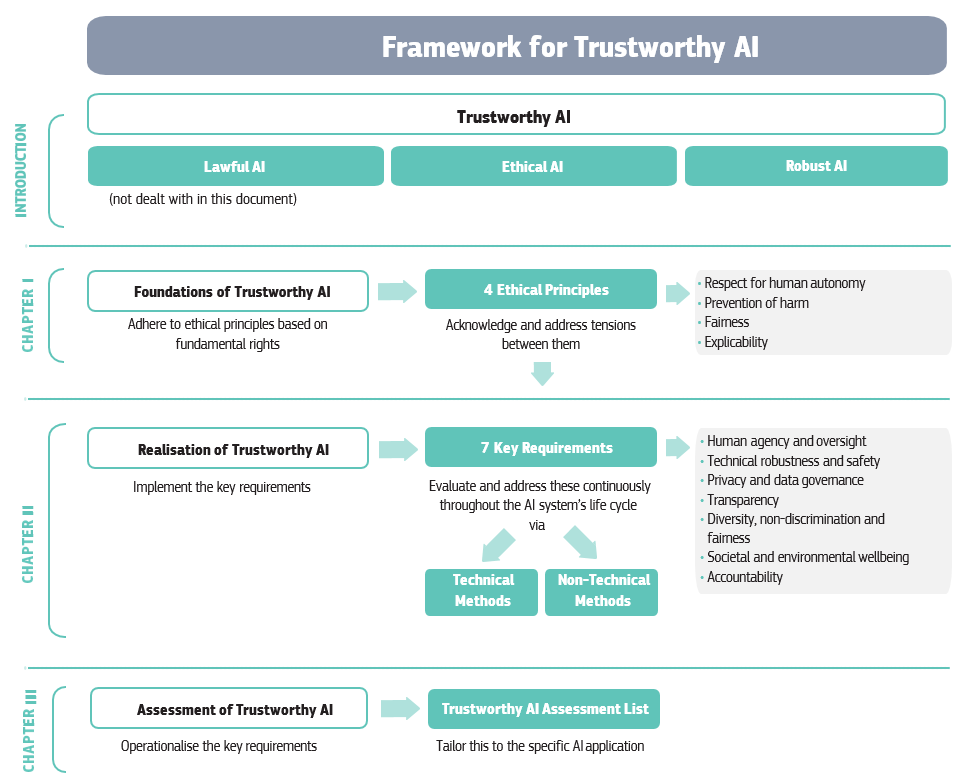
\includegraphics[width=0.9\linewidth]{./img/hleg_ethics_guidelines.png}
    \caption{General overview of the document}
\end{figure}


\subsection{Chapter I: Foundations of trustworthy AI} \label{sec:hleg_ch1}

The concept of AI ethics presented in the framework is rooted to the fundamental rights described in the EU Treaties, EU Charter, and international human rights laws.

\begin{remark}[Fundamental rights]
    \phantom{}
    \begin{itemize}
        \item Respect human dignity as moral subjects rather than objects in the pipeline of the system. AI systems should protect humans' physical and mental integrity, personal and cultural identity, and essential needs.
        \item Guarantee individual's freedom such as freedom of business, of the arts and science, of expression, of assembly, and the right of privacy. AI systems should be mitigated for coercion, threats, surveillance, deception, \dots
        \item Guarantee equality, non-discrimination, and solidarity. The output of an AI system should not be biased. Vulnerable groups that risk exclusion should be respected.
        \item Respect for democracy and citizen's rights. AI systems should not undermine democratic processes or citizen's rights such as the right to vote, to access public documents, to petition, \dots
    \end{itemize}
\end{remark}

\begin{remark}
    Seen as legally enforceable rights, fundamental rights can be considered as part of the \textsc{lawful} AI component. Seen as the rights of everyone, from a moral status, they fall within the \textsc{ethical} AI component.
\end{remark}

This chapter describes four ethical principle for trustworthy AI based on fundamental rights:
\begin{descriptionlist}
    \item[Principle of respect for human autonomy] \marginnote{Principle of respect for human autonomy}
        AI users should keep full self-determination. AI systems should be human-centric leaving room for human choices and they should not manipulate them.

        % AI should empower individuals and not control and restrict freedom. Vulnerable groups need extra protection.
    
    \item[Principle of prevention of harm] \marginnote{Principle of prevention of harm}
        AI systems should operate in technically robust and safe environments. Attention must be paid to groups vulnerable to exclusion and to those subject to power asymmetries (e.g., employer-employee).
        % Address negative impacts by defining mitigation measures based on the risk level.

        % \begin{remark}
        %     There might be unforeseen risks.
        % \end{remark}

    \item[Principle of fairness] \marginnote{Principle of fairness}
        The concept of fairness is described in a substantive and procedural dimension. The substantive dimension implies unbiased outputs and an equal distribution between benefits and costs. The procedural dimension involves the ability to contest and correct decisions made by AI systems and by humans using them.

        % Ensure unbiased outputs guarantying equal treatment and avoiding discriminations.

    \item[Principle of explicability] \marginnote{Principle of explicability}
        AI systems need to be transparent, their capabilities and purpose should be communicated, and their decisions should be as explainable as possible. For black box algorithms, alternative explicability measures might be needed (e.g., traceability, auditability, and communication of capabilities). Also, the degree of explicability that is required is dependent on the context and the use case.
\end{descriptionlist}

\begin{remark}
    There might be tensions between these principles (e.g., between prevention of harm and human autonomy in predictive policing) and methods to deal with them have to be established. Overall, the benefits of AI systems should exceed the risks. Practitioners should study these trade-offs in a reasoned and evidence-based way and not solely based on intuition. 
\end{remark}


\subsection{Chapter II: Realization of trustworthy AI} \label{sec:hleg_ch2}

This chapter defines concrete requirements from the principles of \hyperref[sec:hleg_ch1]{Chapter I}. Stakeholders that these requirements involve are:
\begin{descriptionlist}
    \item[Developers] \marginnote{Developers}
        Who research, design, and develop AI systems. They should concretely apply these requirements.

    \item[Deployers] \marginnote{Deployers}
        Who use AI systems in their business processes and offer products or services to others. They should ensure that the systems they use meet the requirements.

    \item[End-users] \marginnote{End-users}
        Who use the final AI system. They should be informed of these requirements and can request that they are respected.
\end{descriptionlist}

The main requirements the framework defines are:
\begin{descriptionlist}
    \item[Human agency and oversight] \marginnote{Human agency and oversight}
        AI systems should enhance human autonomy and decision-making (principle of respect for human autonomy):
        \begin{itemize}
            \item If there is the risk of violating fundamental rights, a study of the impacts should be conducted to justify it. External feedback should also be considered.
            \item Users should be provided with the necessary knowledge and tools to comprehend and interact with AI systems. 
            \item Users have the right to not be subject to only automatic decisions if this significantly affects them.
            \item There should be oversight mechanisms (of varying degrees depending on the risk) to prevent AI systems from undermining human autonomy:
            \begin{itemize}
                \item Human-in-the-loop (HITL): human intervention in every decision.
                \item Human-on-the-loop (HOTL): human intervention in the design cycle and monitoring of the system's operation.
                \item Human-in-command (HIC): human to decide if, when, and how to use an AI system in any particular situation.
            \end{itemize}
            Public enforcers should also have the ability to exercise oversight with proper authorizations.
        \end{itemize}

    \item[Technical robustness and safety] \marginnote{Technical robustness and safety}
        There should be preventative measures to minimize unintentional harm (principle of prevention of harm):
        \begin{itemize}
            \item AI systems should be protected against vulnerabilities and attacks that target the data (data poisoning), the model (model leakage), or the infrastructure.
            \item Possible unintended uses or abuse of the system should be taken into account and mitigated.
            \item There should be fallback plans in case of problems (e.g., switching from a statistical to a rule-based algorithm, asking a human, \dots).
            \item There should be an explicit evaluation process to assess the accuracy of the AI system and determine its error rate.
            \item The output of an AI system should be reliable (robust to a wide range of inputs) and reproducible.
        \end{itemize}

    \item[Privacy and data governance] \marginnote{Privacy and data governance}
        Quality and security of the data should be guaranteed through the lifecycle of the AI system (principle of prevention of harm):
        \begin{itemize}
            \item Data provided by the user and derived from it should be protected and not used unlawfully or unfairly.
            \item Datasets should be cleared from biases, inaccuracies, and errors before training.
            \item The integrity of the datasets must be ensured to prevent malicious attacks.
            \item Processes and datasets should be tested and documented.
        \end{itemize}

        % AI must protect users' private data. Decisions should be traceable.

    \item[Transparency] \marginnote{Transparency}
        There should be transparency in all the elements of an AI system (principle of explicability):
        \begin{itemize}
            \item The construction process of the dataset and the processes that lead to the AI system's decision should be documented.
            \item Decisions made by an AI system should be understandable and traceable by a human.
            \item The reason to use an AI system and the degree to which it influences decision-making and design choices should be stated.
            \item AI systems should not present themselves as humans and users have the right to be informed if they are interacting with an AI system. Depending on the use case, there should be the option to interact with a human.
            \item Capabilities and limitations of an AI system should be communicated to practitioners or end-users.
        \end{itemize}

        % Decision making process should be explainable.

    \item[Diversity, non-discrimination, and fairness] \marginnote{Diversity, non-discrimination, and fairness}
        Inclusion and diversity should be considered in the entire lifecycle of an AI system (principle of fairness):
        \begin{itemize}
            \item Biases should be removed from the data during the collection phase. Oversight processes should be put in place.
            \item AI systems should be user-centric and designed to be accessible by all people, regardless of disabilities.
            \item Stakeholders who might be affected by the AI system should be consulted.
        \end{itemize}

        % AI should be inclusive and not discriminative.

        % Universal design principles (accessibility)

    \item[Societal and environmental well-being] \marginnote{Societal and environmental well-being}
        The impact of AI systems should also consider society in general and the environment (principles of fairness and prevention of harm):
        \begin{itemize}
            \item The environmental impact of the lifecycle of an AI system should be assessed.
            \item The effects of AI systems on people's physical and mental well-being, as well as institutions, democracy, and society should be assessed and monitored.
        \end{itemize}
        % AI should not have negative impacts on the society and environment.

    \item[Accountability] \marginnote{Accountability}
        Clear responsibilities should be defined for decisions made by AI systems (principle of fairness):
        \begin{itemize}
            \item Internal or external auditors should assess algorithms, data, and design processes.
            \item Potential negative impacts of AI systems should be identified, assessed, documented, and minimized.
            \item When there is tension between some of these requirements, trade-offs should be studied methodologically.
            \item There should be a redress mechanism for unjust decisions made by AI systems.
        \end{itemize}
\end{descriptionlist}

The chapter also describes some technical and non-technical methods to ensure trustworthy AI:
\begin{description}
    \item[Technical methods] \marginnote{Technical methods}
        \begin{description}
            \item[Architecture for trustworthy AI] 
                Embed trustworthiness requirements into the AI system as procedures or constraints.

            \item[Ethics and rule of law by design] 
                Methods to provide some properties by design.

            \item[Explanation methods] 
                Use techniques to understand the underlying mechanisms.

            \item[Testing and validating] 
                Define tests and validate the system in its entire lifecycle.

            \item[Quality of service indicators] 
                Use indicators to set the baseline for a trustworthy AI.
        \end{description}


    \item[Non-technical methods] \marginnote{Non-technical methods}
        \begin{description}
            \item[Regulation] 
                Revise, adapt, or introduce regulations.

            \item[Codes of conduct] 
                Describe how the organization intends to use AI systems.

            \item[Standardization] 
                Define standards for a trustworthy system.

            \item[Certification] 
                Create organizations to attest that an AI system is trustworthy.

            \item[Accountability via governance frameworks] 
                Organizations should appoint a person or a board for decisions regarding ethics.

            \item[Education and awareness] 
                Educate, and train involved stakeholders.

            \item[Stakeholder participation and social dialogue] 
                Ensure open discussions between stakeholders and involve the general public.

            \item[Diversity and inclusive design teams] 
                The team working on an AI system should reflect the diversity of users and society.
        \end{description}
\end{description}



% \begin{description}
%     \item[Research and innovation]
%         Assessment and training. Share discoveries with the community.

%     \item[Clear communication]
%         Set expectations for the AI system.

%     \item[Traceability]
%         Tracking and documenting AI decisions, training data, system updates, \dots

%     \item[Stakeholder involvement]
%         Include inputs from diverse Stakeholders: users, policymakers, industry experts, lawyers, \dots
% \end{description}


\subsection{Chapter III Assessment of trustworthy AI} \label{sec:hleg_ch3}

This chapter defines a generic assessment list to implement the requirements of \hyperref[sec:hleg_ch2]{Chapter II}. The list has been devised by first taking feedback from a small selection of companies, organizations, and institutions that implemented it. Then, it was extended to all stakeholders and another round of feedback was taken.

\begin{description}
    \item[Assessment list] \marginnote{Assessment list}
        Steps to concretely assess the trustworthiness of an AI system. The main considerations to take into account are that:
        \begin{itemize}
            \item It should be tailored based on the specific use case.
            \item It can be integrated into existing governance mechanisms.
            \item It is continuously improved.
        \end{itemize}

        \begin{remark}
            In its pilot version, the list is composed of a series of questions for each requirement described in \hyperref[sec:hleg_ch2]{Chapter II}.
        \end{remark}
\end{description}


% EU Commission for AI:
% \begin{itemize}
%     \item Increase public and private funding,
%     \item Prepare society (e.g., protect workers that are substituted with AI),
%     \item Strengthen European values.
% \end{itemize}




% \begin{description}
%     \item[Human-centric AI] 
%         AI to enhance human welfare and freedom. Maximize the potential of AI while minimizing its risks.
% \end{description}






% \begin{description}
%     \item[Guidelines for trustworthy AI]
%         Voluntary ethical framework to provide an approach of developing AI.
% \end{description}



% \begin{description}
%     \item[EU primary law] 
%         EU treaties and fundamental right.

%     \item[EU secondary law] 
%         EU regulations.

%     \item[International treaties]
%         UN human rights treaties and Council of Europe conventions.

%     \item[Member states laws] 
% \end{description}

% \begin{remark}
%     AI must comply to a multi-layered legal framework.
% \end{remark}


% Ethical foundations in AI are based on fundamental values: human dignity, freedoms (business, expression), respect for democracy.

% Equality, non-discrimination, and solidarity.

% No interference with democracy: vote, transparency, access to public documents, right to petition.



% Full self-determination



% \subsection{Principle of fairness}


% \subsection{Principle of explicability}

